% Options for packages loaded elsewhere
% Options for packages loaded elsewhere
\PassOptionsToPackage{unicode}{hyperref}
\PassOptionsToPackage{hyphens}{url}
\PassOptionsToPackage{dvipsnames,svgnames,x11names}{xcolor}
%
\documentclass[
  letterpaper,
  DIV=11,
  numbers=noendperiod]{scrartcl}
\usepackage{xcolor}
\usepackage{amsmath,amssymb}
\setcounter{secnumdepth}{-\maxdimen} % remove section numbering
\usepackage{iftex}
\ifPDFTeX
  \usepackage[T1]{fontenc}
  \usepackage[utf8]{inputenc}
  \usepackage{textcomp} % provide euro and other symbols
\else % if luatex or xetex
  \usepackage{unicode-math} % this also loads fontspec
  \defaultfontfeatures{Scale=MatchLowercase}
  \defaultfontfeatures[\rmfamily]{Ligatures=TeX,Scale=1}
\fi
\usepackage{lmodern}
\ifPDFTeX\else
  % xetex/luatex font selection
\fi
% Use upquote if available, for straight quotes in verbatim environments
\IfFileExists{upquote.sty}{\usepackage{upquote}}{}
\IfFileExists{microtype.sty}{% use microtype if available
  \usepackage[]{microtype}
  \UseMicrotypeSet[protrusion]{basicmath} % disable protrusion for tt fonts
}{}
\makeatletter
\@ifundefined{KOMAClassName}{% if non-KOMA class
  \IfFileExists{parskip.sty}{%
    \usepackage{parskip}
  }{% else
    \setlength{\parindent}{0pt}
    \setlength{\parskip}{6pt plus 2pt minus 1pt}}
}{% if KOMA class
  \KOMAoptions{parskip=half}}
\makeatother
% Make \paragraph and \subparagraph free-standing
\makeatletter
\ifx\paragraph\undefined\else
  \let\oldparagraph\paragraph
  \renewcommand{\paragraph}{
    \@ifstar
      \xxxParagraphStar
      \xxxParagraphNoStar
  }
  \newcommand{\xxxParagraphStar}[1]{\oldparagraph*{#1}\mbox{}}
  \newcommand{\xxxParagraphNoStar}[1]{\oldparagraph{#1}\mbox{}}
\fi
\ifx\subparagraph\undefined\else
  \let\oldsubparagraph\subparagraph
  \renewcommand{\subparagraph}{
    \@ifstar
      \xxxSubParagraphStar
      \xxxSubParagraphNoStar
  }
  \newcommand{\xxxSubParagraphStar}[1]{\oldsubparagraph*{#1}\mbox{}}
  \newcommand{\xxxSubParagraphNoStar}[1]{\oldsubparagraph{#1}\mbox{}}
\fi
\makeatother


\usepackage{longtable,booktabs,array}
\newcounter{none} % for unnumbered tables
\usepackage{calc} % for calculating minipage widths
% Correct order of tables after \paragraph or \subparagraph
\usepackage{etoolbox}
\makeatletter
\patchcmd\longtable{\par}{\if@noskipsec\mbox{}\fi\par}{}{}
\makeatother
% Allow footnotes in longtable head/foot
\IfFileExists{footnotehyper.sty}{\usepackage{footnotehyper}}{\usepackage{footnote}}
\makesavenoteenv{longtable}
\usepackage{graphicx}
\makeatletter
\newsavebox\pandoc@box
\newcommand*\pandocbounded[1]{% scales image to fit in text height/width
  \sbox\pandoc@box{#1}%
  \Gscale@div\@tempa{\textheight}{\dimexpr\ht\pandoc@box+\dp\pandoc@box\relax}%
  \Gscale@div\@tempb{\linewidth}{\wd\pandoc@box}%
  \ifdim\@tempb\p@<\@tempa\p@\let\@tempa\@tempb\fi% select the smaller of both
  \ifdim\@tempa\p@<\p@\scalebox{\@tempa}{\usebox\pandoc@box}%
  \else\usebox{\pandoc@box}%
  \fi%
}
% Set default figure placement to htbp
\def\fps@figure{htbp}
\makeatother

\ifLuaTeX
  \usepackage{luacolor}
  \usepackage[soul]{lua-ul}
\else
  \usepackage{soul}
\fi

% definitions for citeproc citations
\NewDocumentCommand\citeproctext{}{}
\NewDocumentCommand\citeproc{mm}{%
  \begingroup\def\citeproctext{#2}\cite{#1}\endgroup}
\makeatletter
 % allow citations to break across lines
 \let\@cite@ofmt\@firstofone
 % avoid brackets around text for \cite:
 \def\@biblabel#1{}
 \def\@cite#1#2{{#1\if@tempswa , #2\fi}}
\makeatother
\newlength{\cslhangindent}
\setlength{\cslhangindent}{1.5em}
\newlength{\csllabelwidth}
\setlength{\csllabelwidth}{3em}
\newenvironment{CSLReferences}[2] % #1 hanging-indent, #2 entry-spacing
 {\begin{list}{}{%
  \setlength{\itemindent}{0pt}
  \setlength{\leftmargin}{0pt}
  \setlength{\parsep}{0pt}
  % turn on hanging indent if param 1 is 1
  \ifodd #1
   \setlength{\leftmargin}{\cslhangindent}
   \setlength{\itemindent}{-1\cslhangindent}
  \fi
  % set entry spacing
  \setlength{\itemsep}{#2\baselineskip}}}
 {\end{list}}
\usepackage{calc}
\newcommand{\CSLBlock}[1]{\hfill\break\parbox[t]{\linewidth}{\strut\ignorespaces#1\strut}}
\newcommand{\CSLLeftMargin}[1]{\parbox[t]{\csllabelwidth}{\strut#1\strut}}
\newcommand{\CSLRightInline}[1]{\parbox[t]{\linewidth - \csllabelwidth}{\strut#1\strut}}
\newcommand{\CSLIndent}[1]{\hspace{\cslhangindent}#1}



\setlength{\emergencystretch}{3em} % prevent overfull lines

\providecommand{\tightlist}{%
  \setlength{\itemsep}{0pt}\setlength{\parskip}{0pt}}



 


\KOMAoption{captions}{tableheading}
\makeatletter
\@ifpackageloaded{tcolorbox}{}{\usepackage[skins,breakable]{tcolorbox}}
\@ifpackageloaded{fontawesome5}{}{\usepackage{fontawesome5}}
\definecolor{quarto-callout-color}{HTML}{909090}
\definecolor{quarto-callout-note-color}{HTML}{0758E5}
\definecolor{quarto-callout-important-color}{HTML}{CC1914}
\definecolor{quarto-callout-warning-color}{HTML}{EB9113}
\definecolor{quarto-callout-tip-color}{HTML}{00A047}
\definecolor{quarto-callout-caution-color}{HTML}{FC5300}
\definecolor{quarto-callout-color-frame}{HTML}{acacac}
\definecolor{quarto-callout-note-color-frame}{HTML}{4582ec}
\definecolor{quarto-callout-important-color-frame}{HTML}{d9534f}
\definecolor{quarto-callout-warning-color-frame}{HTML}{f0ad4e}
\definecolor{quarto-callout-tip-color-frame}{HTML}{02b875}
\definecolor{quarto-callout-caution-color-frame}{HTML}{fd7e14}
\makeatother
\makeatletter
\@ifpackageloaded{caption}{}{\usepackage{caption}}
\AtBeginDocument{%
\ifdefined\contentsname
  \renewcommand*\contentsname{Table of contents}
\else
  \newcommand\contentsname{Table of contents}
\fi
\ifdefined\listfigurename
  \renewcommand*\listfigurename{List of Figures}
\else
  \newcommand\listfigurename{List of Figures}
\fi
\ifdefined\listtablename
  \renewcommand*\listtablename{List of Tables}
\else
  \newcommand\listtablename{List of Tables}
\fi
\ifdefined\figurename
  \renewcommand*\figurename{Figure}
\else
  \newcommand\figurename{Figure}
\fi
\ifdefined\tablename
  \renewcommand*\tablename{Table}
\else
  \newcommand\tablename{Table}
\fi
}
\@ifpackageloaded{float}{}{\usepackage{float}}
\floatstyle{ruled}
\@ifundefined{c@chapter}{\newfloat{codelisting}{h}{lop}}{\newfloat{codelisting}{h}{lop}[chapter]}
\floatname{codelisting}{Listing}
\newcommand*\listoflistings{\listof{codelisting}{List of Listings}}
\makeatother
\makeatletter
\makeatother
\makeatletter
\@ifpackageloaded{caption}{}{\usepackage{caption}}
\@ifpackageloaded{subcaption}{}{\usepackage{subcaption}}
\makeatother
\usepackage{bookmark}
\IfFileExists{xurl.sty}{\usepackage{xurl}}{} % add URL line breaks if available
\urlstyle{same}
\hypersetup{
  pdftitle={MECO4114 Research Methods},
  pdfauthor={Francesco Bailo},
  colorlinks=true,
  linkcolor={blue},
  filecolor={Maroon},
  citecolor={Blue},
  urlcolor={Blue},
  pdfcreator={LaTeX via pandoc}}


\title{MECO4114 Research Methods}
\usepackage{etoolbox}
\makeatletter
\providecommand{\subtitle}[1]{% add subtitle to \maketitle
  \apptocmd{\@title}{\par {\large #1 \par}}{}{}
}
\makeatother
\subtitle{Week 04 Digital Research Methods}
\author{Francesco Bailo}
\date{2026-03-18}
\begin{document}
\maketitle


\subsection{Acknowledgement of
Country}\label{acknowledgement-of-country}

I would like to acknowledge the Traditional Owners of Australia and
recognise their continuing connection to land, water and culture. The
University of Sydney is located on the land of the Gadigal people of the
Eora Nation. I pay my respects to their Elders, past and present.

\subsection{Who am I}\label{who-am-i}

\textbf{Academic Background}

\begin{itemize}
\tightlist
\item
  PhD in Government \& International Relations (University of Sydney,
  2017)
\item
  Senior Lecturer in the School of Government and International
  Relations, School of Social and Political Sciences
\item
  Co-Director,
  \href{https://www.sydney.edu.au/arts/our-research/centres-institutes-and-groups/centre-for-ai-trust-and-governance.html}{Centre
  for AI, Trust and Governance} and Director of the
  \href{https://canvas.sydney.edu.au/courses/65547}{Computational Social
  Science Lab}
\end{itemize}

\textbf{Research Focus}

\begin{itemize}
\tightlist
\item
  Intersection of digital technologies and political participation, and
  democratic governance
\item
  Computational methods for understanding information systems and their
  societal and political impacts
\end{itemize}

\textbf{Teaching}: GOVT6139 Research Design (S2), SSPS4102/6006 Data
analytics (with R, S1), GOVT3901 Digital Politics (S2) and CISS6022
Cybersecurity (S1).

You can reach me at francesco.bailo@sydney.edu.au.

\section{Observing behaviour}\label{observing-behaviour}

\subsection{}\label{section}

This section is largely based on Chapter 2 of Salganik (2018).

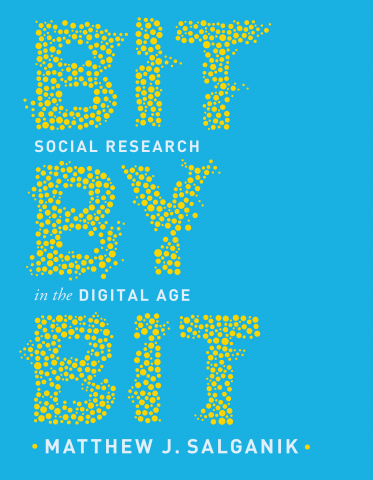
\includegraphics[width=0.7\linewidth,height=\textheight,keepaspectratio]{figure/9780691158648.png}

\subsection{Three ways to collect
data}\label{three-ways-to-collect-data}

Whatever the subject of your research, there are mainly three ways to
collect data:

\begin{enumerate}
\def\labelenumi{\arabic{enumi}.}
\tightlist
\item
  Running experiments
\end{enumerate}

. . .

\begin{enumerate}
\def\labelenumi{\arabic{enumi}.}
\setcounter{enumi}{1}
\tightlist
\item
  Asking questions
\end{enumerate}

. . .

\begin{enumerate}
\def\labelenumi{\arabic{enumi}.}
\setcounter{enumi}{2}
\tightlist
\item
  Observing behaviour \(\leftarrow\)
\end{enumerate}

. . .

\begin{itemize}
\tightlist
\item
  Observational data are collected without interfering with either

  \begin{itemize}
  \tightlist
  \item
    the subject of the investigation or
  \item
    the environment of the subject of the investigation.
  \end{itemize}
\end{itemize}

\subsection{The primordial way of
investigating}\label{the-primordial-way-of-investigating}

Observation of something or somebody is the primordial way of
investigating what we are interested in (and usually the beginning of an
investigation).

Using instruments and sensors to observe and record what we observe is
not new.

What is new is the number of instruments and sensors that monitor and
record human behaviour.

\begin{figure}[H]

{\centering 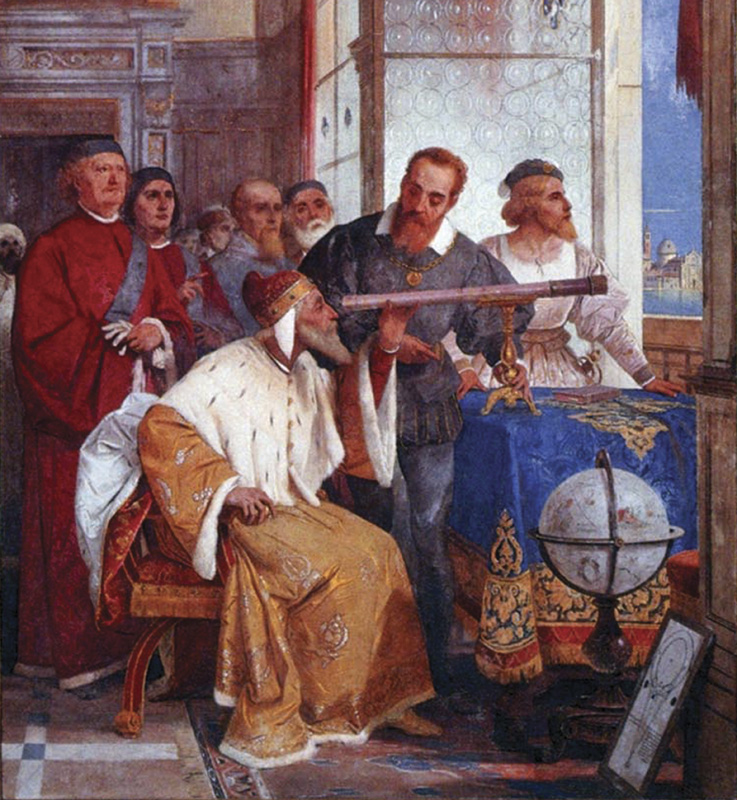
\includegraphics[width=0.7\linewidth,height=\textheight,keepaspectratio,alt={@bertini\_galileo\_1858}]{figure/Bertini_fresco_of_Galileo_Galilei_and_Doge_of_Venice.jpg}

}

\caption{\emph{Bertini (1858)}}

\end{figure}%

\subsection{Big Data}\label{big-data}

The combination of \emph{flow} and the \emph{stock} of data produced by
these instruments and sensors is often called \textbf{Big Data}.

Big data are \emph{big} on three dimensions:

\begin{itemize}
\tightlist
\item
  \textbf{V}olume
\item
  \textbf{V}ariety
\item
  \textbf{V}elocity
\end{itemize}

\subsection{Examples of Big Data}\label{examples-of-big-data}

\begin{itemize}
\item
  So\ldots{} can you think of any example of big data or source of big
  data?
\item
  Big data are not only data generated by the online activity of users
  and are not only created by companies.
\end{itemize}

\begin{enumerate}
\def\labelenumi{\arabic{enumi}.}
\item
  Big data are generated online and offline every time a sensor records
  a human behaviour.
\item
  Big data are created by companies and governments.
\end{enumerate}

\subsection{Big Data: Companies and
Governments}\label{big-data-companies-and-governments}

\begin{quote}
``Big data are created and collected by \textbf{companies} and
\textbf{governments} for purposes other than research. Using this data
for research therefore requires repurposing.'' (Salganik, 2018, p. 14)
\end{quote}


\includegraphics[width=0.5\linewidth,height=\textheight,keepaspectratio]{figure/300px-Twitter_bird_logo_2012.pdf}

\(\neq\)


\includegraphics[width=0.7\linewidth,height=\textheight,keepaspectratio]{figure/640px-ABS_Census_Logo.pdf}

\subsection{Ten characteristics of Big Data
(1/2)}\label{ten-characteristics-of-big-data-12}

According to Salganik (2018), Big Data shares ten characteristics.

\begin{enumerate}
\def\labelenumi{\arabic{enumi}.}
\item
  Big Data are \textbf{big}: Rare events, heterogeneity, small
  differences. \emph{But} how data were created?
\item
  Big Data are \textbf{always-on}: Unexpected events and real-time
  estimates. \emph{But} the systems that collected the data are
  constantly changing (see \emph{drifting} later)!
\item
  Big Data are \textbf{nonreactive}: Measurement is less likely to
  change behaviour. \emph{But} a social desirability bias persists.
\item
  Big Data are \textbf{incomplete}: No demographic information, no
  information on behaviour on other platforms, and no data to
  operationalise theoretical constructs (e.g.~``intelligence'').
\item
  Big Data are \textbf{inaccessible}: Access is controlled and
  conditional.
\end{enumerate}

\subsection{Ten characteristics of Big Data
(2/2)}\label{ten-characteristics-of-big-data-22}

\begin{enumerate}
\def\labelenumi{\arabic{enumi}.}
\setcounter{enumi}{5}
\item
  Big Data are \textbf{non-representative}: Data do not come from a
  probabilistic random population sample.
\item
  Big Data are \textbf{drifting}: Population drift, behavioural drift,
  system drift. Systems keep changing all the time!
\item
  Big Data are \textbf{algorithmically confounded}: Engineering choices
  impact user behaviours. Also, performativity issues.
\item
  Big Data are \textbf{dirty}: Dirty data can be created unintentionally
  or intentionally (e.g.~bots).
\item
  Big Data are \textbf{sensitive}: The potential sensitivity of the data
  is always difficult to assess.
\end{enumerate}

\section{Network analysis}\label{network-analysis}

\subsection{A very short introduction}\label{a-very-short-introduction}

\begin{tcolorbox}[enhanced jigsaw, arc=.35mm, bottomrule=.15mm, bottomtitle=1mm, breakable, colback=white, colbacktitle=quarto-callout-note-color!10!white, colframe=quarto-callout-note-color-frame, coltitle=black, left=2mm, leftrule=.75mm, opacityback=0, opacitybacktitle=0.6, rightrule=.15mm, title=\textcolor{quarto-callout-note-color}{\faInfo}\hspace{0.5em}{Relations, not attributes. Networks, not groups.}, titlerule=0mm, toprule=.15mm, toptitle=1mm]

{[}S{]}ocial network analysts argue that causation is not located in the
individual, but in the social structure. While people with similar
attributes may behave similarly, explaining these similarities by
pointing to common attributes misses the reality that \emph{individuals
with common attributes often occupy similar positions in the social
structure}. That is, \emph{people with similar attributes frequently
have similar social network positions}. Their similar outcomes are
caused by the \textbf{constraints}, \textbf{opportunities} and
\textbf{perceptions} created by these similar network positions. (Marin
\& Wellman, 2011, p. 13)

\end{tcolorbox}

\subsection{Network visualisation and adjacency
matrix}\label{network-visualisation-and-adjacency-matrix}

\begin{figure}[H]

{\centering \pandocbounded{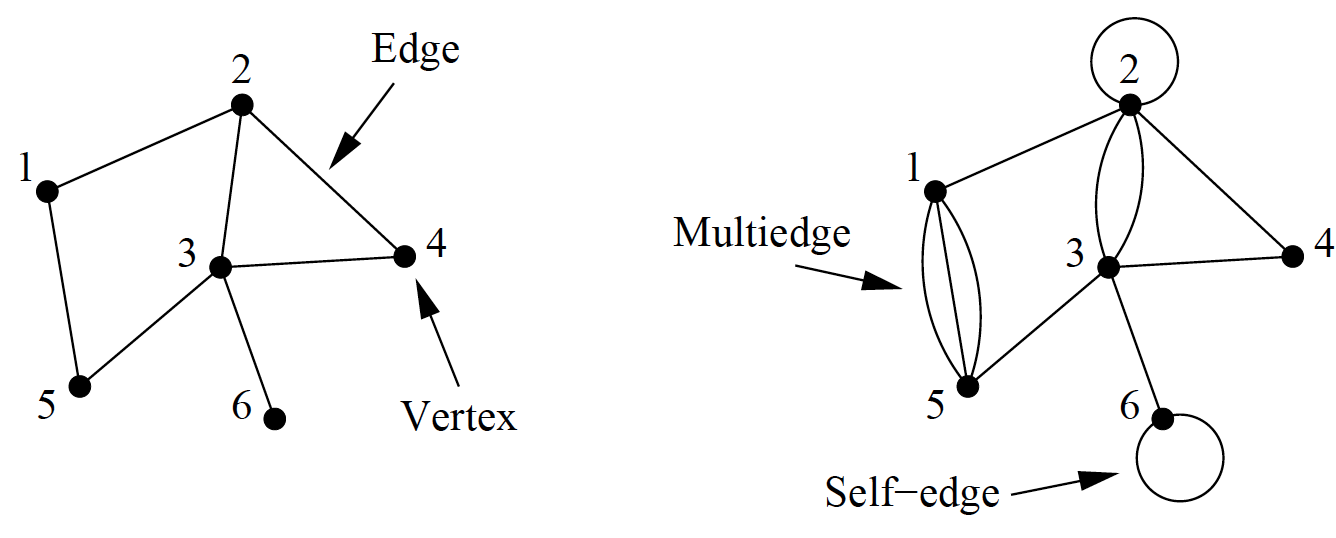
\includegraphics[keepaspectratio,alt={Traditional visualisation of two small networks\ldots{}}]{figure/undirected_network.pdf}}

}

\caption{Traditional visualisation of two small networks\ldots{}}

\end{figure}%

\begin{figure}[H]

{\centering \pandocbounded{\includegraphics[keepaspectratio,alt={\ldots{} and the adjacency matrix of the left-hand network {[}@newman\_networks\_2010, p. 111{]}.}]{figure/undirected_adj_matrix.pdf}}

}

\caption{\ldots{} and the adjacency matrix of the left-hand network
(Newman, 2010, p. 111).}

\end{figure}%

\subsection{Directed networks}\label{directed-networks}

\begin{figure}[H]

{\centering 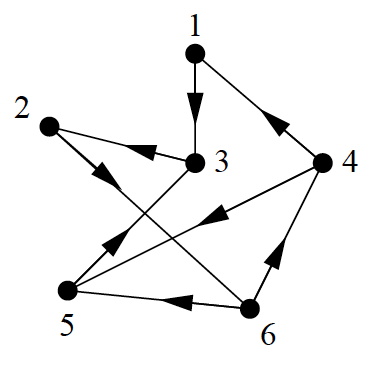
\includegraphics[width=0.7\linewidth,height=\textheight,keepaspectratio,alt={A directed network\ldots{}}]{figure/directed_network.pdf}

}

\caption{A directed network\ldots{}}

\end{figure}%

\begin{figure}[H]

{\centering \pandocbounded{\includegraphics[keepaspectratio,alt={\ldots{} and its adjacency matrix (not symmetric!) {[}@newman\_networks\_2010, p. 112{]}.}]{figure/directed_adj_matrix.pdf}}

}

\caption{\ldots{} and its adjacency matrix (not symmetric!) (Newman,
2010, p. 112).}

\end{figure}%

\subsection{Network measures}\label{network-measures}

\begin{itemize}
\tightlist
\item
  \textbf{Degree of a vertex}: number of connections
\item
  \textbf{Authority of a vertex}: number of important connections
\item
  \textbf{Closeness of a vertex}: mean distance to other vertices
\item
  \textbf{Betweenness of a vertex}: extent to which a vertex lies on
  paths between other vertices
\item
  \textbf{Group of vertices}
\end{itemize}

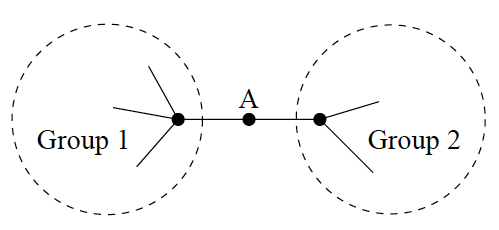
\includegraphics[width=0.55\linewidth,height=\textheight,keepaspectratio]{figure/betweenness.pdf}

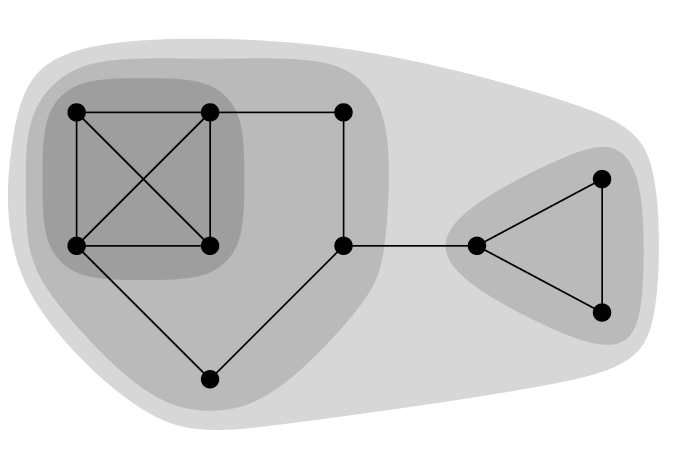
\includegraphics[width=0.55\linewidth,height=\textheight,keepaspectratio]{figure/groups.pdf}

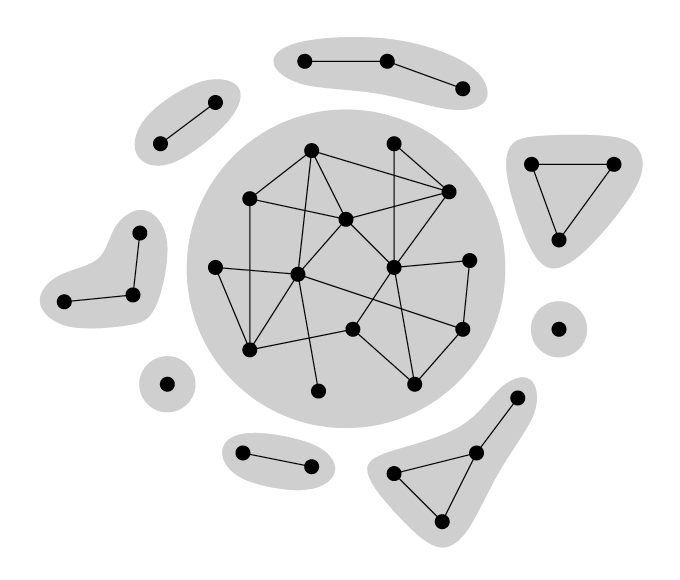
\includegraphics[width=0.55\linewidth,height=\textheight,keepaspectratio]{figure/components.pdf}

\subsection{Network measures
(continued)}\label{network-measures-continued}

\begin{itemize}
\tightlist
\item
  \textbf{Transitivity of edges}: Alice \emph{friend of} Bob
  \emph{friend of} Cat \emph{friend of} Alice
\item
  \textbf{Reciprocity of edges}: Alice \emph{friend of} Bob \emph{friend
  of} Alice
\item
  \textbf{Similarity of vertices}: extent to which the
  \emph{neighbourhood} of vertices is similar
\item
  \textbf{Homophily of vertices}: tendency to associate with similar
  vertices
\end{itemize}

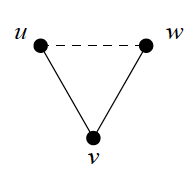
\includegraphics[width=0.35\linewidth,height=\textheight,keepaspectratio]{figure/transitivity.png}

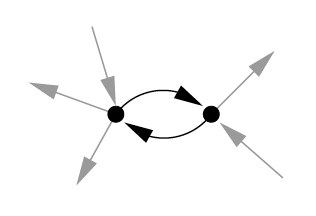
\includegraphics[width=0.4\linewidth,height=\textheight,keepaspectratio]{figure/reciprocity.png}

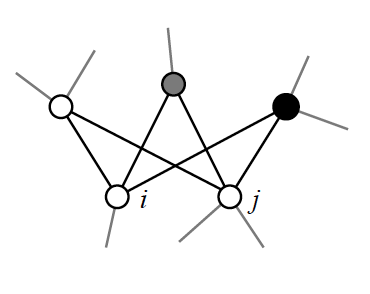
\includegraphics[width=0.4\linewidth,height=\textheight,keepaspectratio]{figure/similarity.png}

\subsection{Example: Friendship
network}\label{example-friendship-network}

\begin{figure}[H]

{\centering \includegraphics[width=0.55\linewidth,height=\textheight,keepaspectratio,alt={Friendship network at a US high school {[}@newman\_networks\_2010, p. 221{]}.}]{figure/race_network.pdf}

}

\caption{Friendship network at a US high school (Newman, 2010, p. 221).}

\end{figure}%

\subsection{Community detection}\label{community-detection}

The goal of a community detection algorithm is simply to separate nodes
into groups that have only a few edges \emph{between} them and many
edges \emph{within}.

\begin{figure}[H]

{\centering 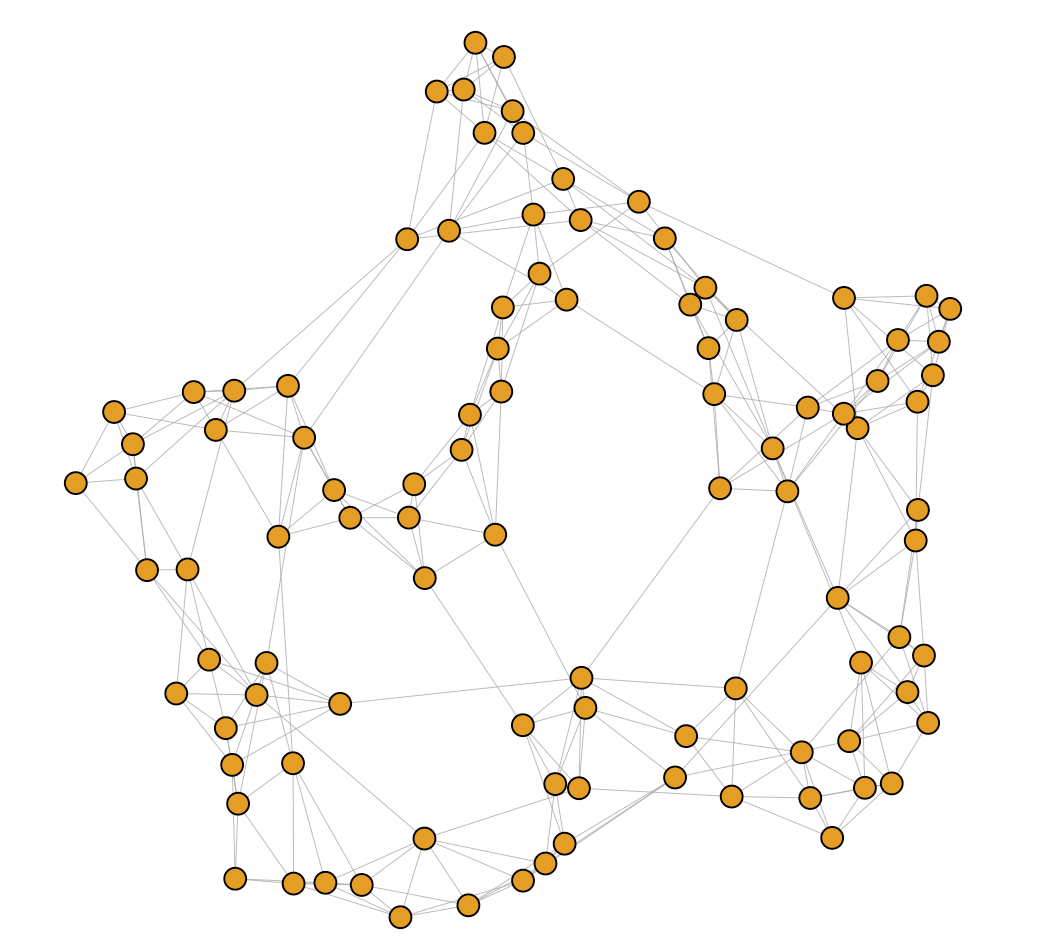
\includegraphics[width=0.4\linewidth,height=\textheight,keepaspectratio,alt={A randomly generated network with 100 vertices and 300 edges}]{figure/sample_smallworld.pdf}

}

\caption{A randomly generated network with 100 vertices and 300 edges}

\end{figure}%

\subsection{Community detection
exercise}\label{community-detection-exercise}

How many communities do you see in this network?

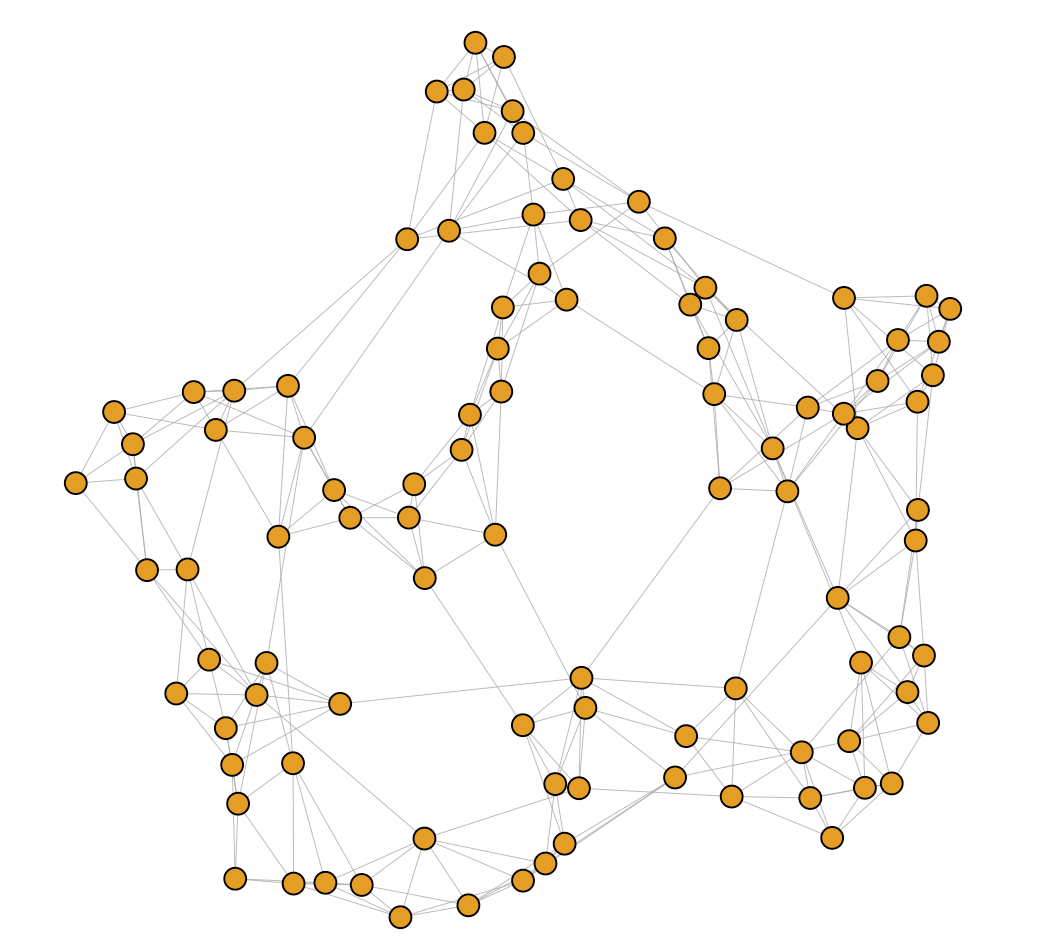
\includegraphics[width=0.4\linewidth,height=\textheight,keepaspectratio]{figure/sample_smallworld.pdf}

\subsection{Community detection
result}\label{community-detection-result}

\pandocbounded{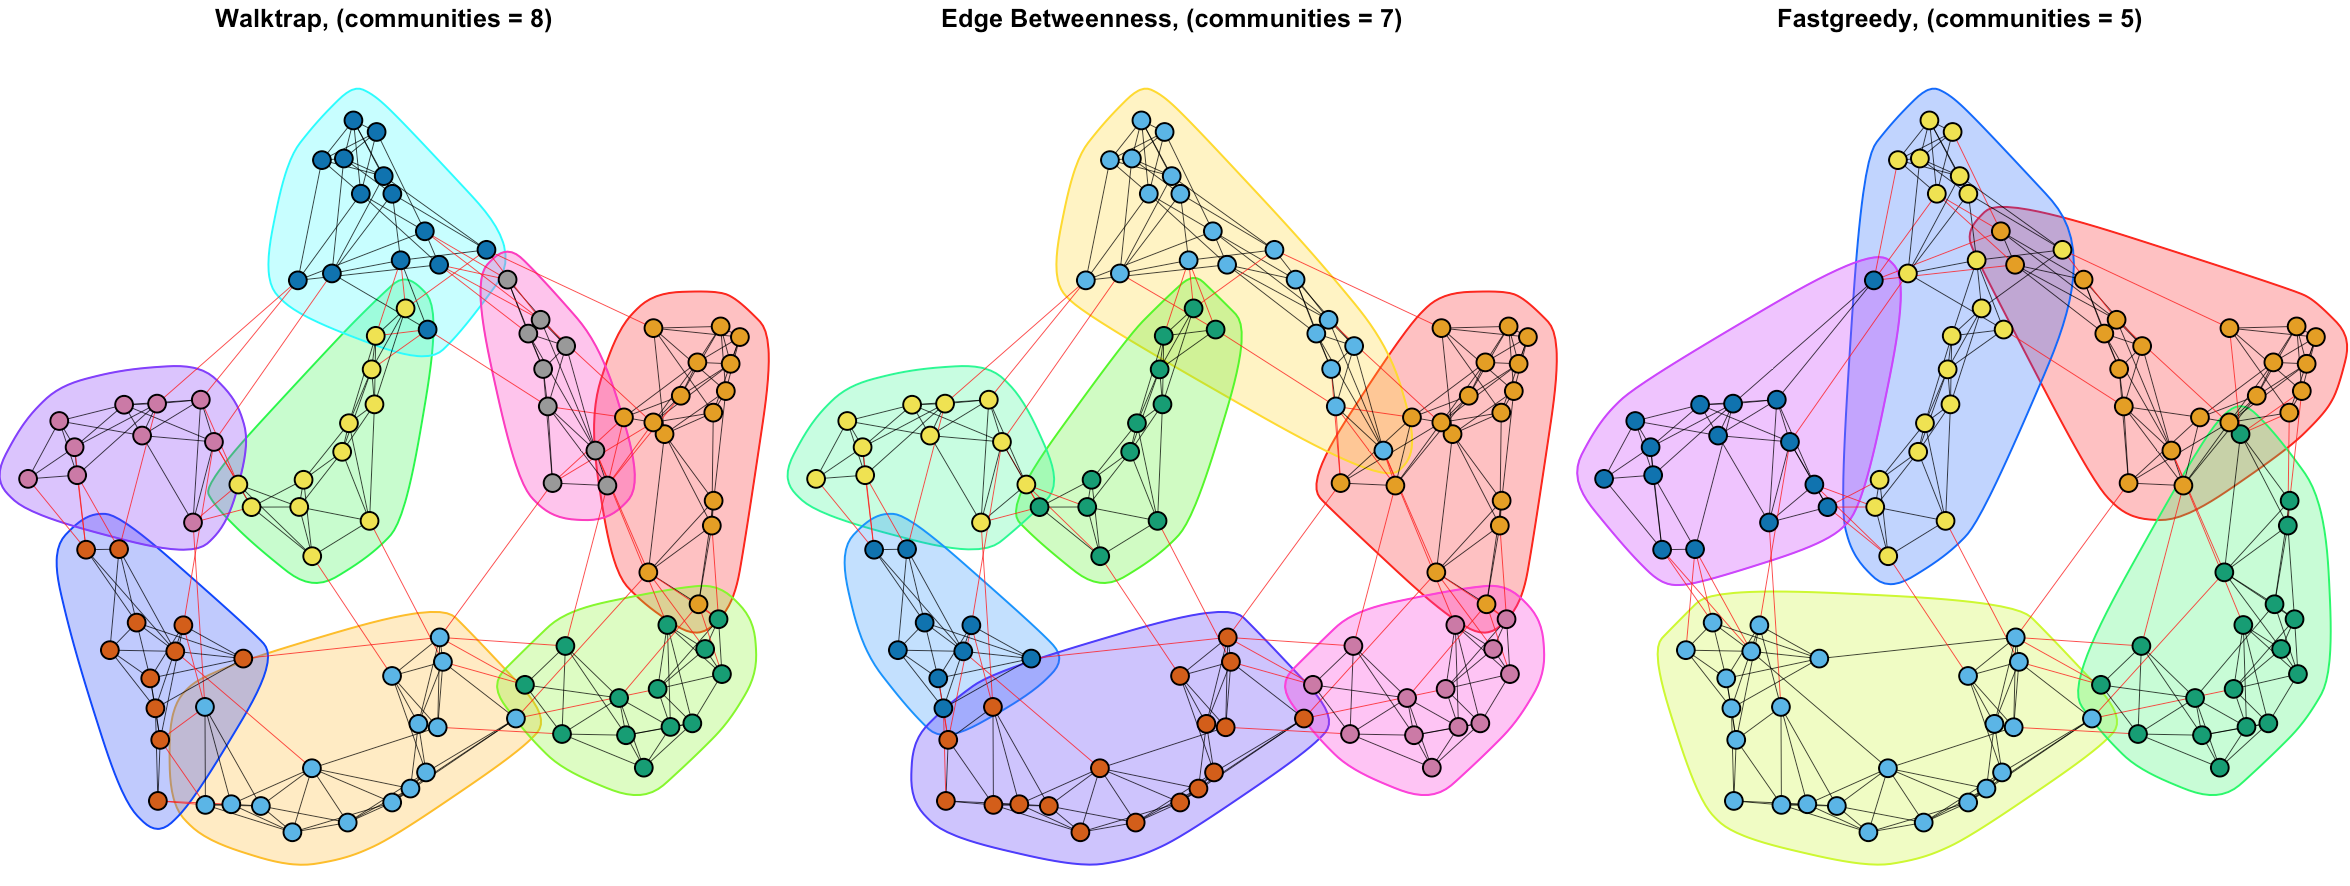
\includegraphics[keepaspectratio]{figure/sample_smallworld_communities.pdf}}

\subsection{Research example}\label{research-example}

\pandocbounded{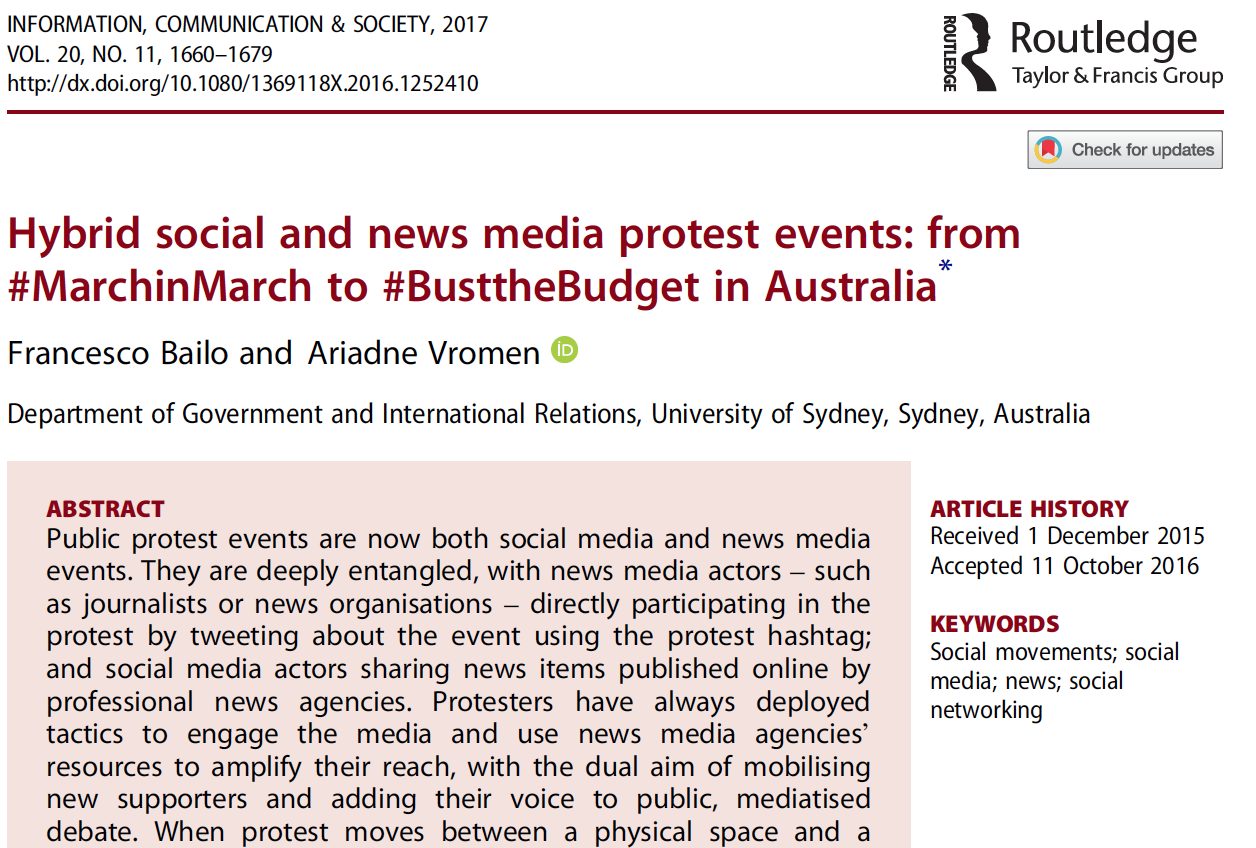
\includegraphics[keepaspectratio]{figure/paper_bailo.pdf}}

\pandocbounded{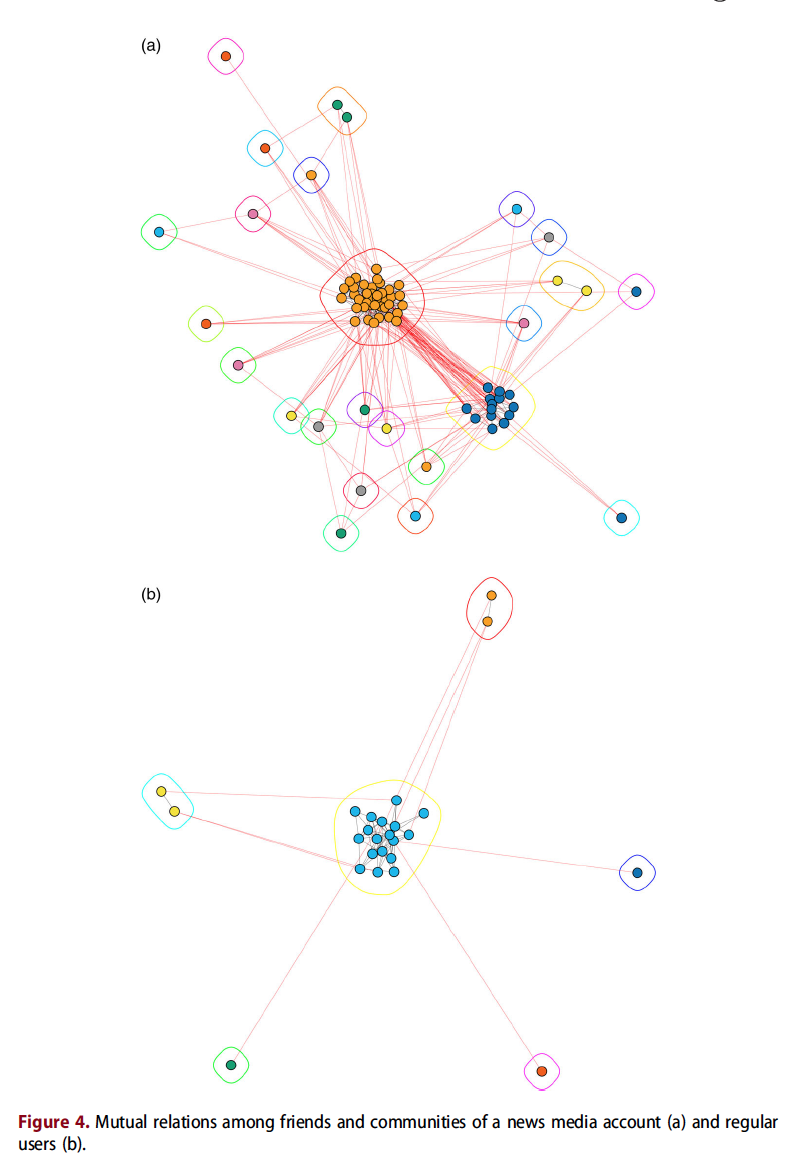
\includegraphics[keepaspectratio]{figure/paper_network.pdf}}

\subsection{Tools for network
analysis}\label{tools-for-network-analysis}

\subsubsection{\texorpdfstring{Easy, small n: Gephi
(\href{https://gephi.org}{gephi.org})}{Easy, small n: Gephi (gephi.org)}}\label{easy-small-n-gephi-gephi.org}

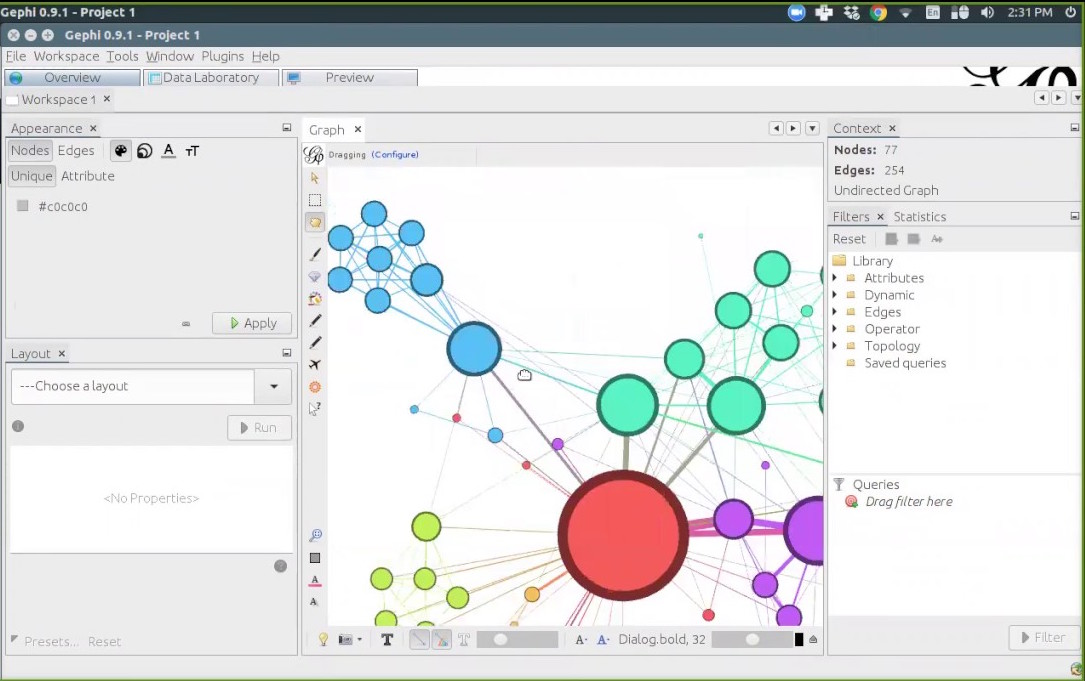
\includegraphics[width=0.65\linewidth,height=\textheight,keepaspectratio]{figure/gephi.jpg}

\subsection{Tools for network analysis
(continued)}\label{tools-for-network-analysis-continued}

\subsubsection{Hard, big n: igraph
package}\label{hard-big-n-igraph-package}

igraph (\href{https://igraph.org}{igraph.org}) in R
(\href{https://www.r-project.org}{www.r-project.org}) or Python
(\href{https://www.python.org}{www.python.org})

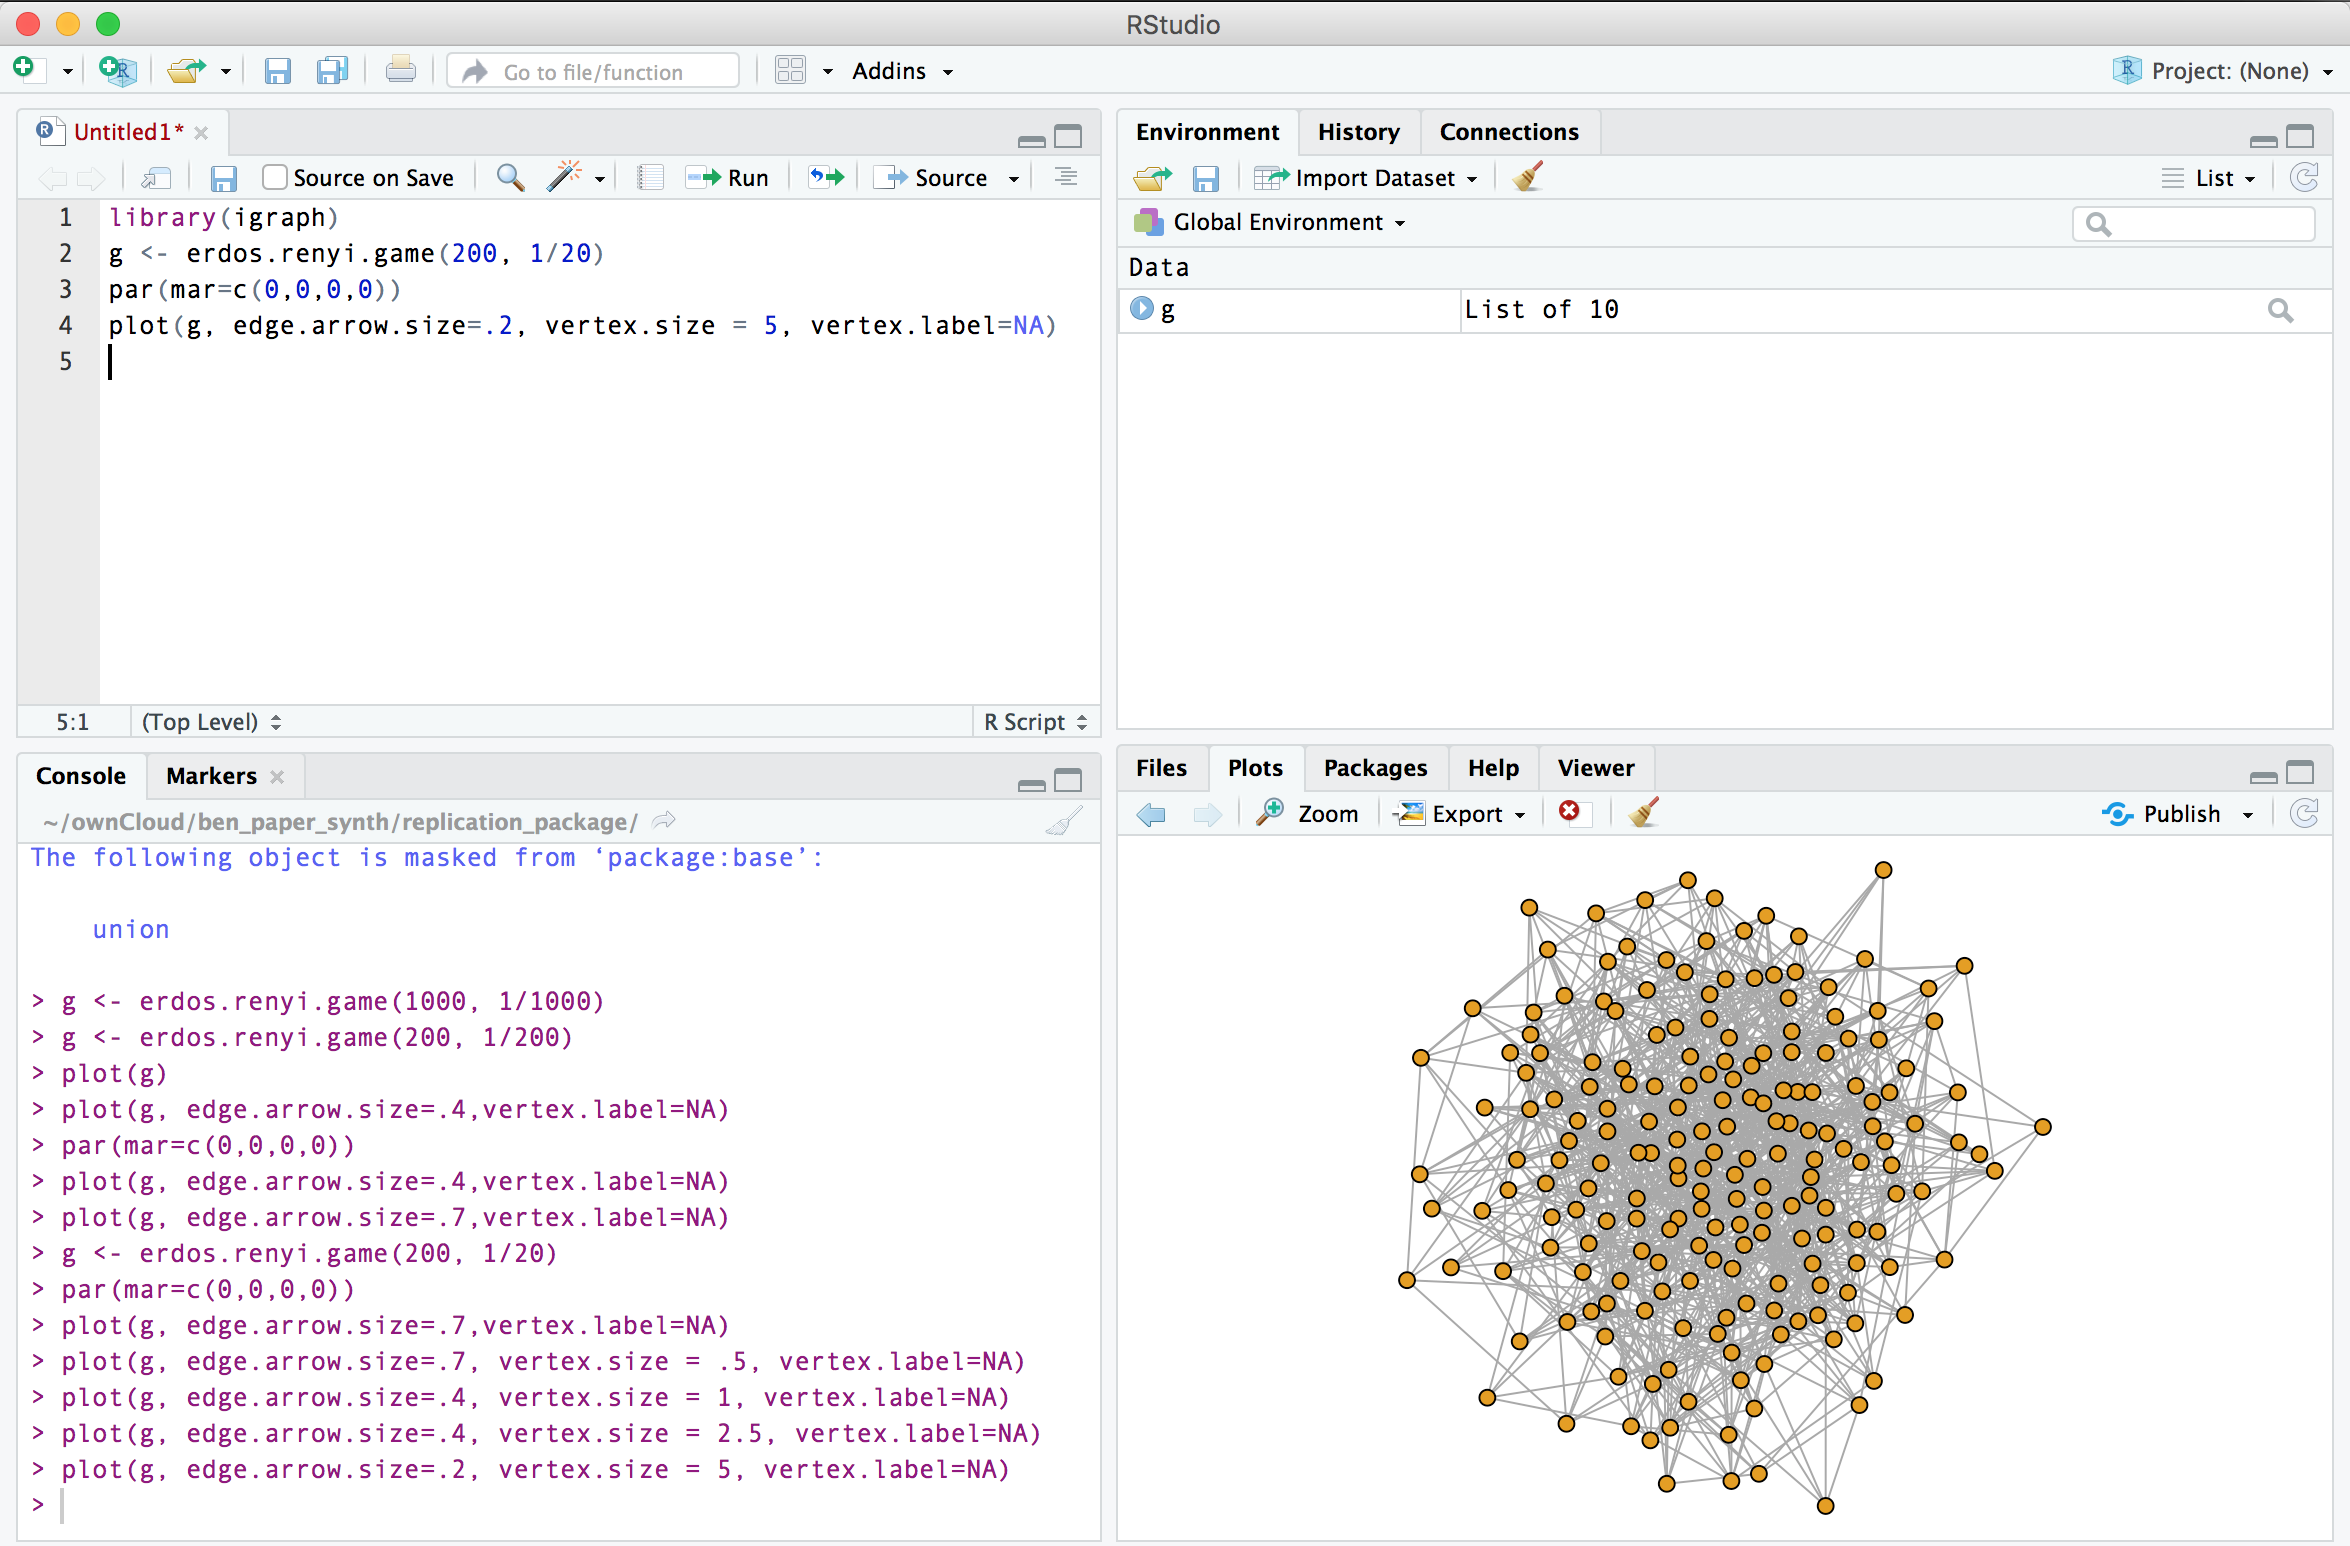
\includegraphics[width=0.6\linewidth,height=\textheight,keepaspectratio]{figure/igraph.pdf}

\subsection{Resources for network
analysis}\label{resources-for-network-analysis}

Getting started bibliography:

\begin{itemize}
\tightlist
\item
  \textbf{Easy}: Scott (2012)
\item
  \textbf{Important}: Marin \& Wellman (2011)
\item
  \textbf{Hard}: Newman (2010)
\end{itemize}

\subsection{Tutorials for beginners}\label{tutorials-for-beginners}

Tutorials for beginners by Katherine Ognyanova (Rutgers University):

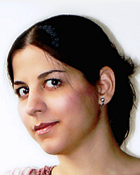
\includegraphics[width=0.1\linewidth,height=\textheight,keepaspectratio]{figure/Ognyanova_Katherine.pdf}

\begin{itemize}
\tightlist
\item
  Network visualisation with Gephi
  (\href{https://kateto.net/sunbelt2016}{kateto.net/sunbelt2016})
\item
  Network visualization with R
  (\href{https://kateto.net/network-visualization}{kateto.net/network-visualization})
\item
  Network Analysis and Visualization with R and igraph
  (\href{https://kateto.net/networks-r-igraph}{kateto.net/networks-r-igraph})
\end{itemize}

\section{Text analysis}\label{text-analysis}

\subsection{Another very short
introduction}\label{another-very-short-introduction}

Quantitative text analysis is necessary when the manual coding of
documents is not feasible or acceptable.

When you face a large \textbf{corpus} of \textbf{documents}, you might
want some methods to automatically:

\begin{enumerate}
\def\labelenumi{\arabic{enumi}.}
\item
  Find patterns within the documents,
\item
  Compare (and maybe group) documents.
\end{enumerate}

\subsection{Finding patterns}\label{finding-patterns}

A textual pattern is as simple as \texttt{dog}.

\begin{itemize}
\item
  Finding patterns doesn't involve any statistical analysis.
\item
  But you might need to use regular expressions (a.k.a. ``regex'') if
  your pattern is complex.
\end{itemize}

\subsection{Finding patterns: Example}\label{finding-patterns-example}

Let's say that you want to find in your corpus all the instances of
\texttt{dog} and \texttt{cat}.

\begin{itemize}
\item
  \textbf{You want to find}: ``I have two \ul{dog}s and a \ul{cat}'' or
  ``\ul{Cat}s are felines''
\item
  \textbf{But you don't want to find}: ``the \ul{cat}egorization of
  syntactic \ul{cat}egories''
\item
  You need a regular expression like:
  \texttt{\textbackslash{}b(cats?\textbar{}dogs?)\textbackslash{}b}
\end{itemize}

{(\href{https://regexr.com/3oqld}{link to interactive example})}

\subsection{Finding patterns: Regex
basics}\label{finding-patterns-regex-basics}

A few simple regex topics:

\begin{itemize}
\tightlist
\item
  \textbf{Quantifier}: \texttt{?}

  \begin{itemize}
  \tightlist
  \item
    \texttt{abc?} matches a string that has ``ab'' followed by zero or
    one ``c''
  \end{itemize}
\item
  \textbf{OR operator}: \texttt{\textbar{}}

  \begin{itemize}
  \tightlist
  \item
    \texttt{a(b\textbar{}c)} matches a string that has ``a'' followed by
    ``b'' or ``c''
  \end{itemize}
\item
  \textbf{Boundaries}: \texttt{\textbackslash{}b}

  \begin{itemize}
  \tightlist
  \item
    \texttt{\textbackslash{}babc\textbackslash{}b} matches only a whole
    word
  \end{itemize}
\end{itemize}

{Exercise: Go to \href{https://regexr.com/3os9b}{regexr.com/3os9b} (not
with Explorer) and enter a regular expression to match ``France'' but
also ``French''.}

\subsection{Comparing documents}\label{comparing-documents}

Comparing documents involves statistical analysis and matrix algebra
(while finding patterns doesn't). It usually relies on Natural-language
processing (NLP), the branch of computer science that studies the human
language and its interactions with the machines.

In its most primordial application, NLP treats documents as
\textbf{bag-of-words} (BoW):

\begin{itemize}
\tightlist
\item
  The \emph{position} of terms within the document is disregarded,
\item
  What counts is the \emph{frequency} of the terms.
\end{itemize}

\subsection{Comparing documents: Processing
steps}\label{comparing-documents-processing-steps}

Let's see how we process documents in a common NLP application.

\begin{itemize}
\item
  We remove from the documents all the stop-words;
\item
  doc1 = ``drugs hospitals doctors'' doc2 = ``smog pollution
  environment'' doc3 = ``doctors hospitals healthcare'' doc4 =
  ``pollution environment water''
\item
  We count the frequency of each term in each document, and we produce a
  term-document matrix
\end{itemize}

\subsection{Comparing documents: Term-document
matrix}\label{comparing-documents-term-document-matrix}

\begin{longtable}[]{@{}lllll@{}}
\caption{Term-document matrix. Terms were stemmed.}\tabularnewline
\toprule\noalign{}
& doc1 & doc2 & doc3 & doc4 \\
\midrule\noalign{}
\endfirsthead
\toprule\noalign{}
& doc1 & doc2 & doc3 & doc4 \\
\midrule\noalign{}
\endhead
\bottomrule\noalign{}
\endlastfoot
doctor & 1 & 0 & 1 & 0 \\
drug & 1 & 0 & 0 & 0 \\
environ & 0 & 1 & 0 & 1 \\
healthcar & 0 & 0 & 1 & 0 \\
hospit & 1 & 0 & 1 & 0 \\
pollut & 0 & 1 & 0 & 1 \\
smog & 0 & 1 & 0 & 0 \\
water & 0 & 0 & 0 & 1 \\
\end{longtable}

\subsection{Bag of Words (BoW)}\label{bag-of-words-bow}

\begin{itemize}
\tightlist
\item
  \textbf{Concept:} Text representation as a bag of its words, ignoring
  the order.
\item
  \textbf{Representation:} Fixed-length vectors, counting word
  occurrences or indicating presence/absence.
\item
  \textbf{Advantages:} Simple, good for specific tasks like spam
  detection.
\item
  \textbf{Limitations:} Ignores context and semantics, leading to
  sparse, high-dimensional vectors.
\end{itemize}

\subsection{Embeddings (used by Large Language
Models)}\label{embeddings-used-by-large-language-models}

\begin{itemize}
\tightlist
\item
  \textbf{Concept:} Dense, low-dimensional vectors representing words,
  capturing semantic meanings.
\item
  \textbf{Representation:} Continuous vectors that reflect context and
  relationships between words.
\item
  \textbf{Advantages:} Captures semantics, reduces dimensionality and is
  versatile for various NLP tasks.
\item
  \textbf{Limitations:} Requires more computational resources, less
  intuitive.
\end{itemize}

\subsection{Tools for text analysis}\label{tools-for-text-analysis}

\begin{itemize}
\item
  Nvivo
  (\href{https://www.qsrinternational.com/nvivo}{www.qsrinternational.com/nvivo})
\item
  Regular Expression (\href{https://regexr.com}{regexr.com})
\item
  R (\href{https://www.r-project.org}{www.r-project.org}) or Python
  (\href{https://www.python.org}{www.python.org})
\item
  ChatGPT and other Large Language Models\ldots{}
\end{itemize}

\subsection{Resources for text
analysis}\label{resources-for-text-analysis}

\begin{itemize}
\item
  \textbf{Introductory}: Jockers (2014)
\item
  \textbf{Introductory}: Bird et al. (2009)
\item
  \textbf{Hard}: Manning et al. (2008)
\end{itemize}

\section{Ethics}\label{ethics}

\subsection{Issues with relational
data}\label{issues-with-relational-data}

\begin{figure}[H]

{\centering \pandocbounded{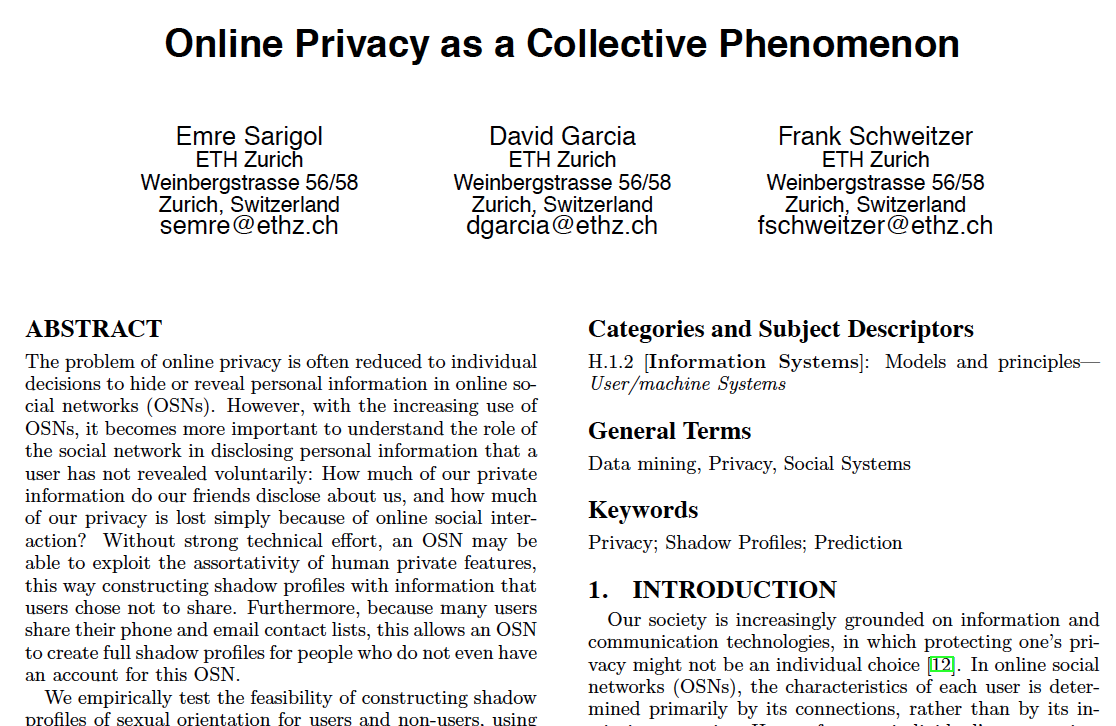
\includegraphics[keepaspectratio,alt={@sarigol\_online\_2014}]{figure/garcia_paper.pdf}}

}

\caption{Sarigol et al. (2014)}

\end{figure}%

\pandocbounded{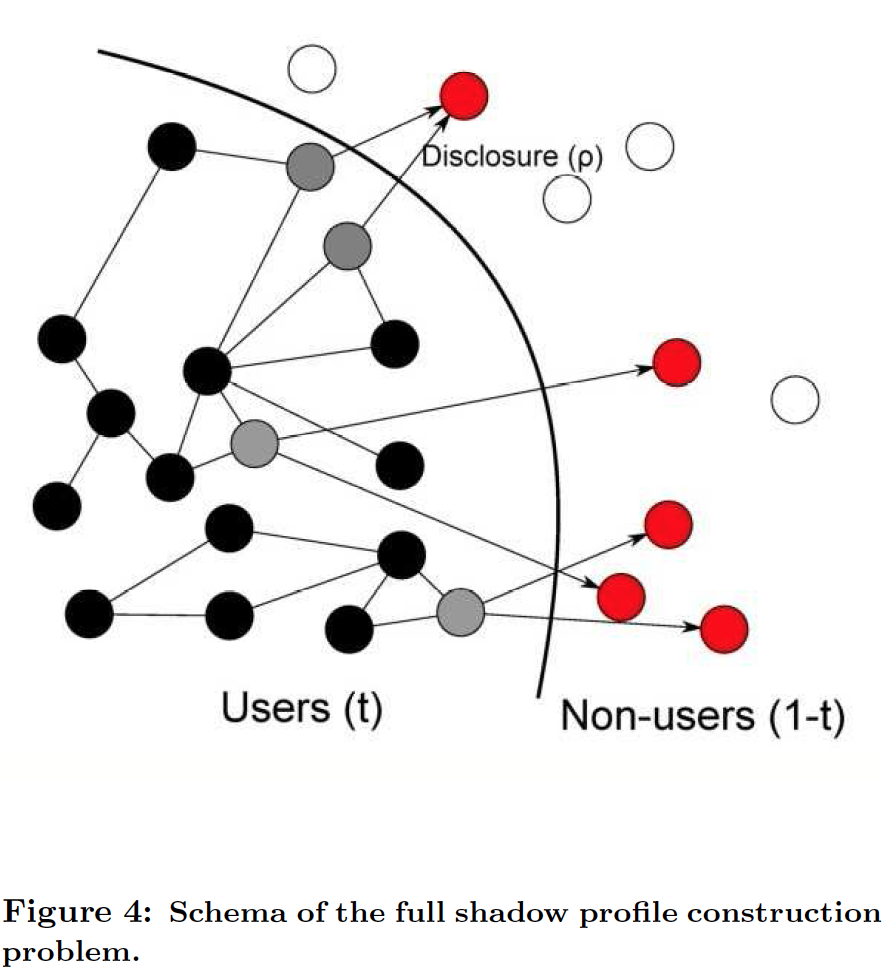
\includegraphics[keepaspectratio]{figure/garcia_fig1.pdf}}

\pandocbounded{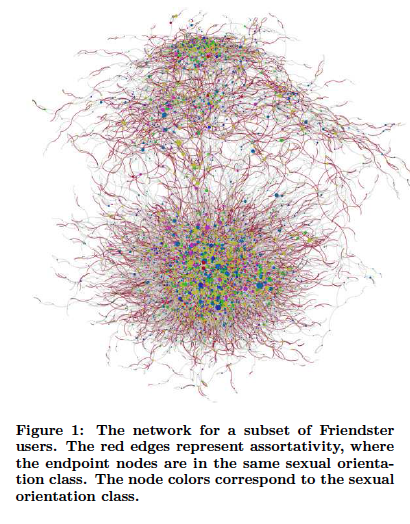
\includegraphics[keepaspectratio]{figure/garcia_fig2.pdf}}

\subsection{Ethics in the digital age: Open
issues}\label{ethics-in-the-digital-age-open-issues}

\begin{itemize}
\item
  Public and Private space. What about online fora (e.g.~Facebook public
  pages?)
\item
  Informed consent.
\item
  Right to privacy. But who owns the data?
\end{itemize}

\section{My research on social media}\label{my-research-on-social-media}

\subsection{Recent publications}\label{recent-publications}

\begin{itemize}
\tightlist
\item
  Kong et al. (2022)
\item
  Bailo et al. (2024)
\item
  Johns et al. (2024)
\end{itemize}

\subsection{Slipping to the extreme}\label{slipping-to-the-extreme}

Kong et al. (2022)

\begin{itemize}
\tightlist
\item
  This study addresses the infiltration of extreme opinions in online
  discussions, leveraging machine learning algorithms alongside
  qualitative research methods.
\item
  Aims to bridge the gap between depth of qualitative insights and
  breadth of quantitative analysis in understanding problematic online
  speech.
\end{itemize}

\subsection{Methodology}\label{methodology}

\begin{itemize}
\tightlist
\item
  Initial qualitative study constructs an ontology of problematic
  speech, identifying key themes and opinions in social media posts.
\item
  Large-scale data collection from Facebook, Twitter, and YouTube,
  followed by iterative dataset augmentation using a human-in-the-loop
  approach.
\item
  Machine learning models classify and augment the dataset, expanding
  the initial qualitative study's findings.
\end{itemize}

\subsection{Research diagram}\label{research-diagram}

\pandocbounded{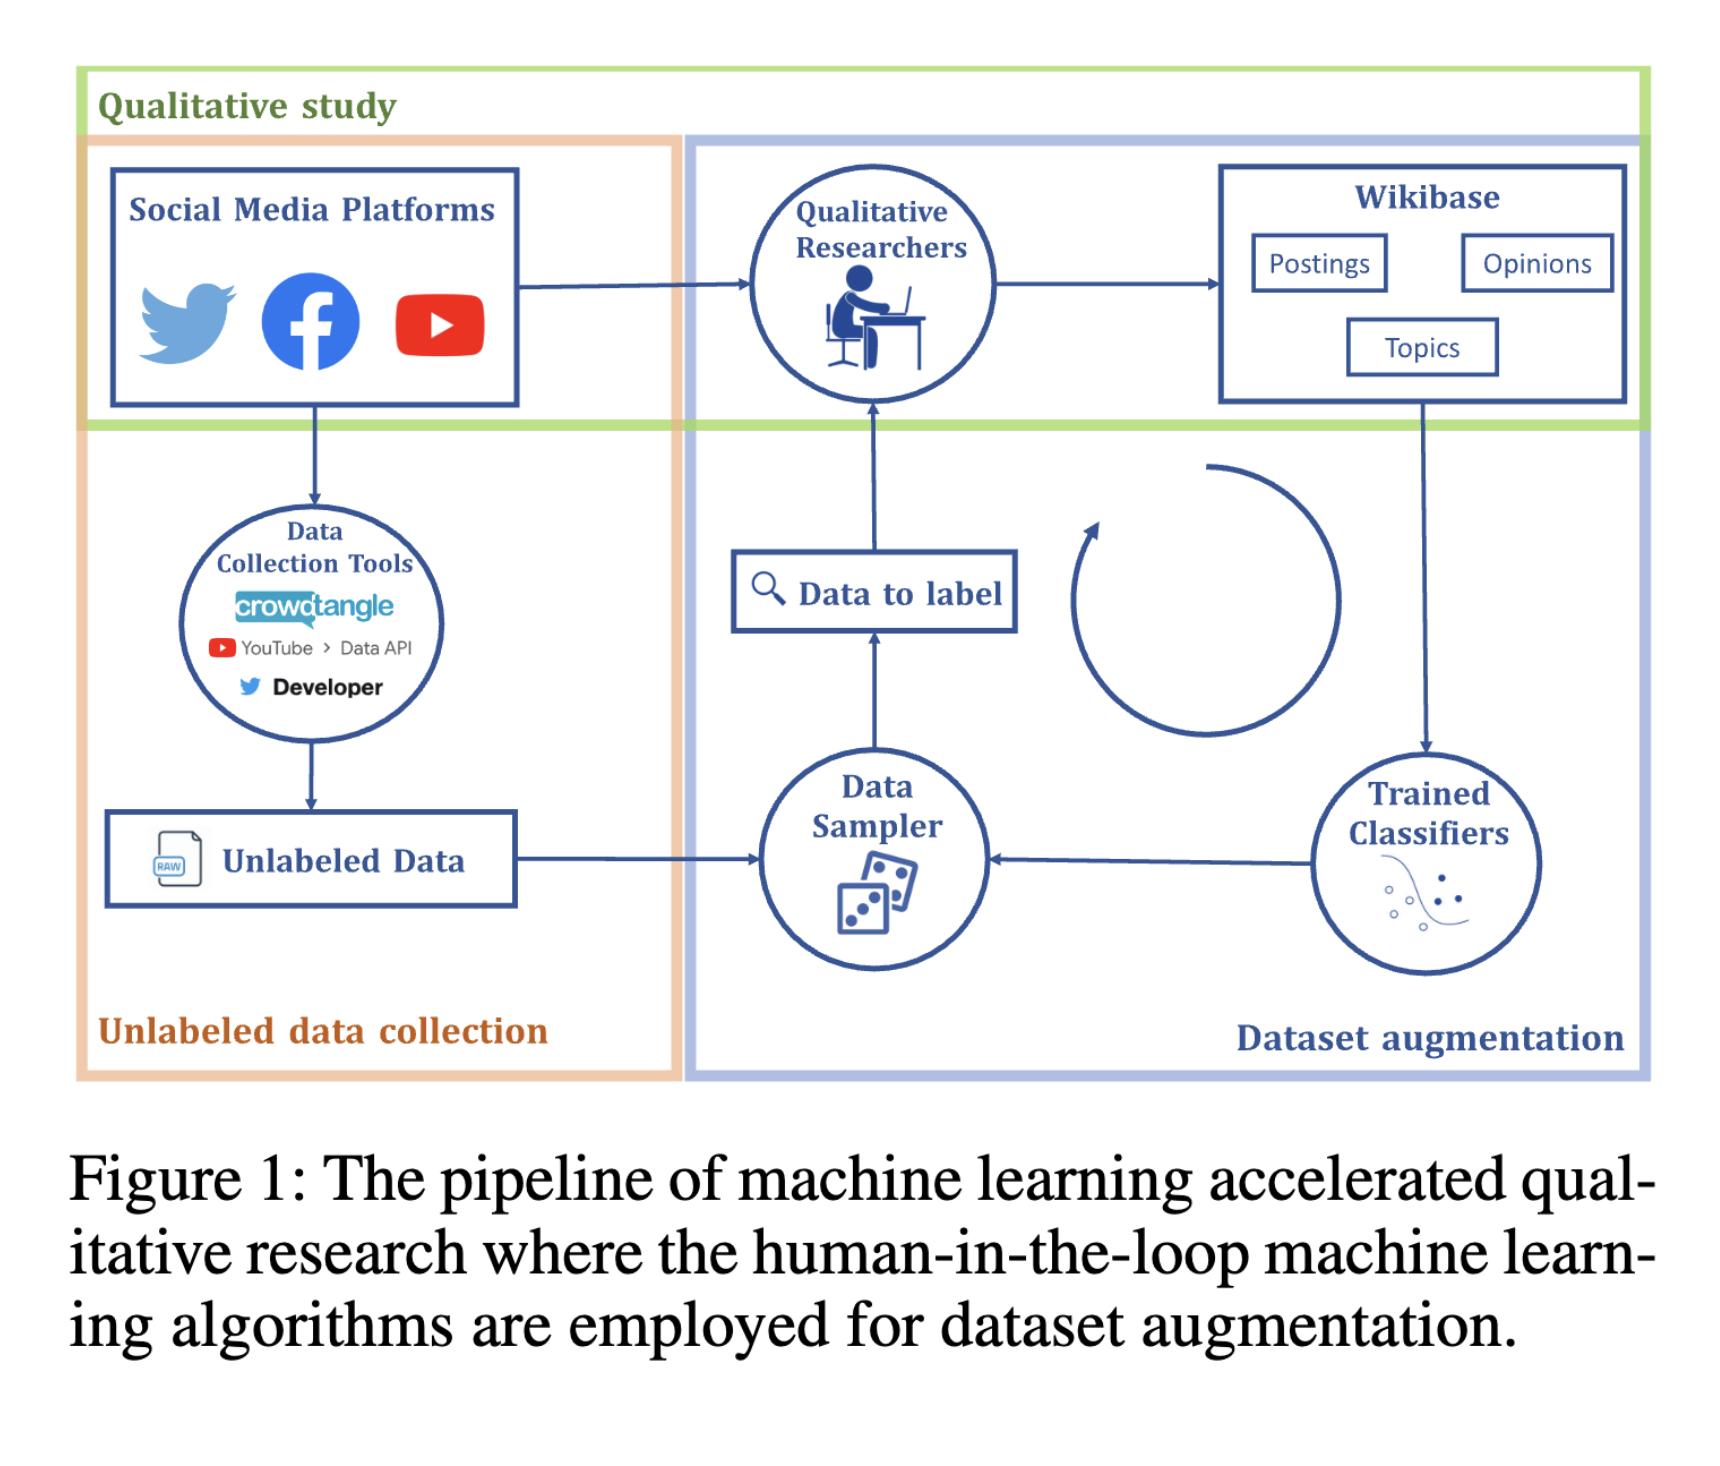
\includegraphics[keepaspectratio]{figure/kongSlippingExtremeMixed2022-fig1.png}}

\subsection{Findings}\label{findings}

\begin{itemize}
\tightlist
\item
  The mixed-method approach successfully identifies and expands the
  dataset, revealing detailed case studies of problematic speech
  dynamics in specific online communities.
\item
  Analysis of opinion emergence and co-occurrence suggests pathways
  through which extreme opinions enter mainstream online discourse.
\end{itemize}

\subsection{Labelling, shadow bans and community
resistance}\label{labelling-shadow-bans-and-community-resistance}

Johns et al. (2024)

\begin{itemize}
\tightlist
\item
  Focus on the effectiveness of Meta's content moderation on Facebook
  during COVID-19.
\item
  Analysis of 18 Australian right-wing/anti-vaccination pages between
  January 2019 and July 2021.
\item
  Integration of engagement metrics, time series analysis, and content
  analysis.
\end{itemize}

\subsection{Sampling}\label{sampling}

\begin{itemize}
\tightlist
\item
  Utilised CrowdTangle to collect data from 21 identified Australian
  Facebook public accounts.
\item
  Final analysis included 18 accounts after excluding those with less
  than 1\% of relevant posts.
\item
  A total of 34,202 postings were analysed.
\end{itemize}

\subsection{Data Analysis}\label{data-analysis}

\begin{itemize}
\tightlist
\item
  Performance analysis via CrowdTangle's `overperforming score' and
  average number of shares-per-post.
\item
  Content and thematic analysis on comments from two overperforming
  public pages.
\item
  Latent Dirichlet Allocation (LDA) for topic modelling and exploration.
\end{itemize}

\subsection{Results visualization}\label{results-visualization}

\pandocbounded{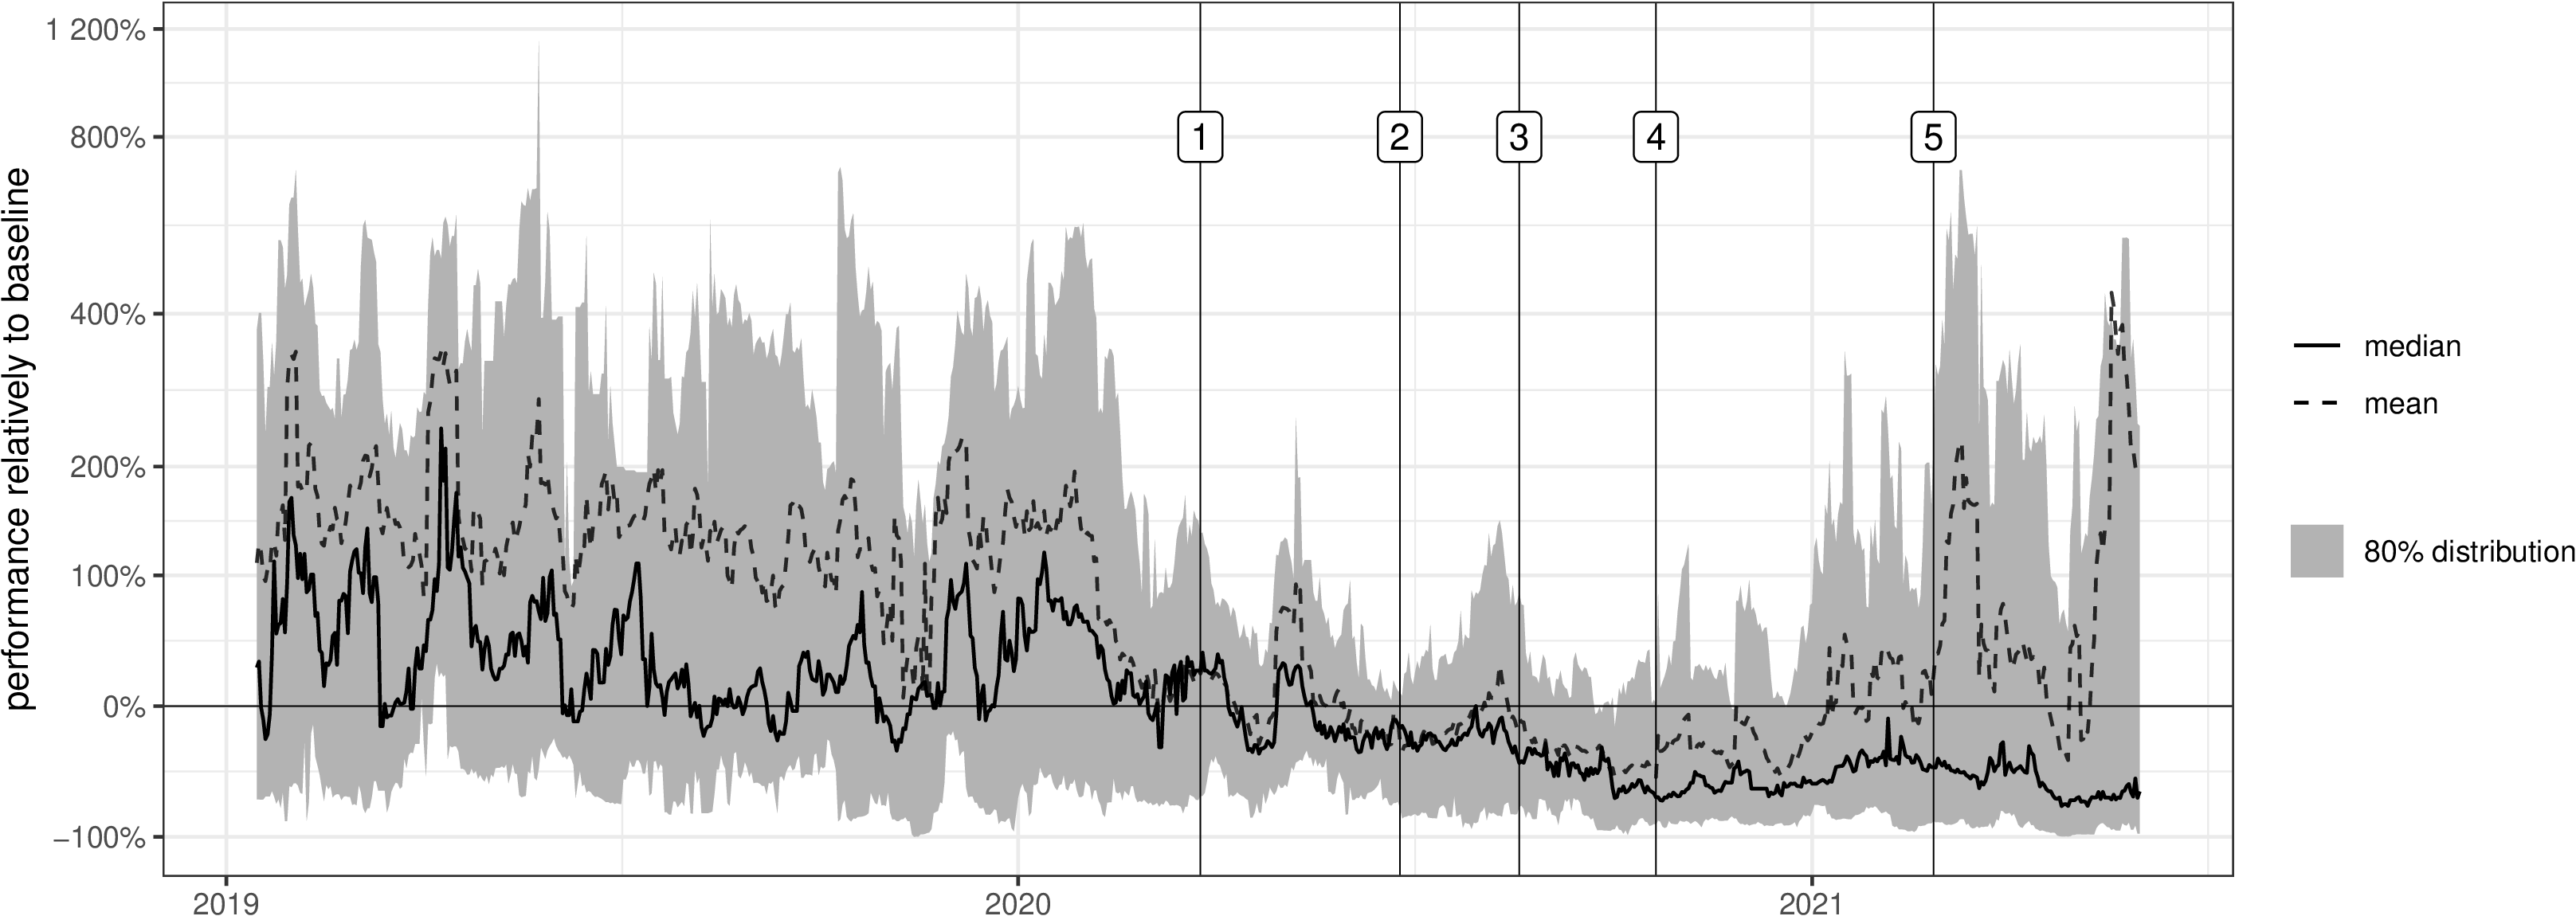
\includegraphics[keepaspectratio]{figure/figure4-1.png}}

\subsection{Policy Review}\label{policy-review}

\begin{itemize}
\tightlist
\item
  Examination of Meta's content moderation and recommendation policy
  announcements.
\item
  Focus on policies introduced from January 2020 to July 2021 relevant
  to Facebook.
\item
  Analysis juxtaposed against key policy announcements and page
  performance.
\end{itemize}

\subsection{Key Findings}\label{key-findings}

\begin{itemize}
\tightlist
\item
  Meta's content moderation systems showed partial effectiveness.
\item
  Identified trends in content labelling and `shadow banning' resistance
  by communities.
\item
  Highlighted the importance and challenges of transparent and
  consistent moderation policies.
\end{itemize}

\section{Bonus: Spatial analysis}\label{bonus-spatial-analysis}

\subsection{Spatial analysis: John Snow's cholera
map}\label{spatial-analysis-john-snows-cholera-map}

\pandocbounded{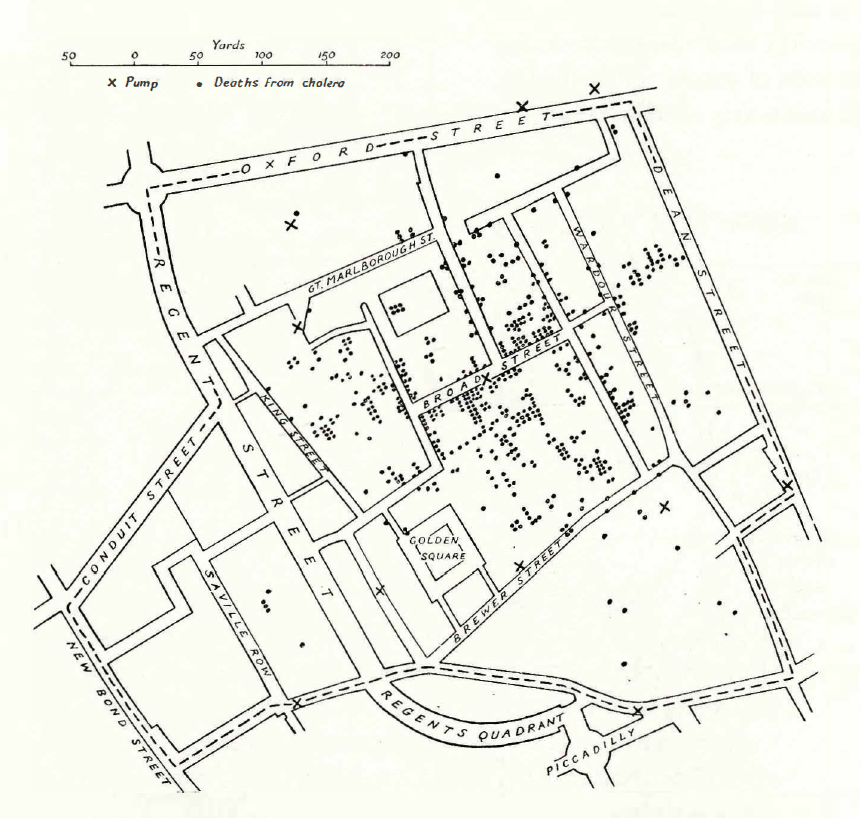
\includegraphics[keepaspectratio]{figure/john_snow_map.pdf}}

Redrawing of John Snow's map of cases of cholera during the London
outbreak of 1854 (Tufte, 2001, p. 24)

\subsection{Tool for spatial analysis}\label{tool-for-spatial-analysis}

\begin{itemize}
\tightlist
\item
  QGIS (\href{https://qgis.org}{qgis.org})
\end{itemize}

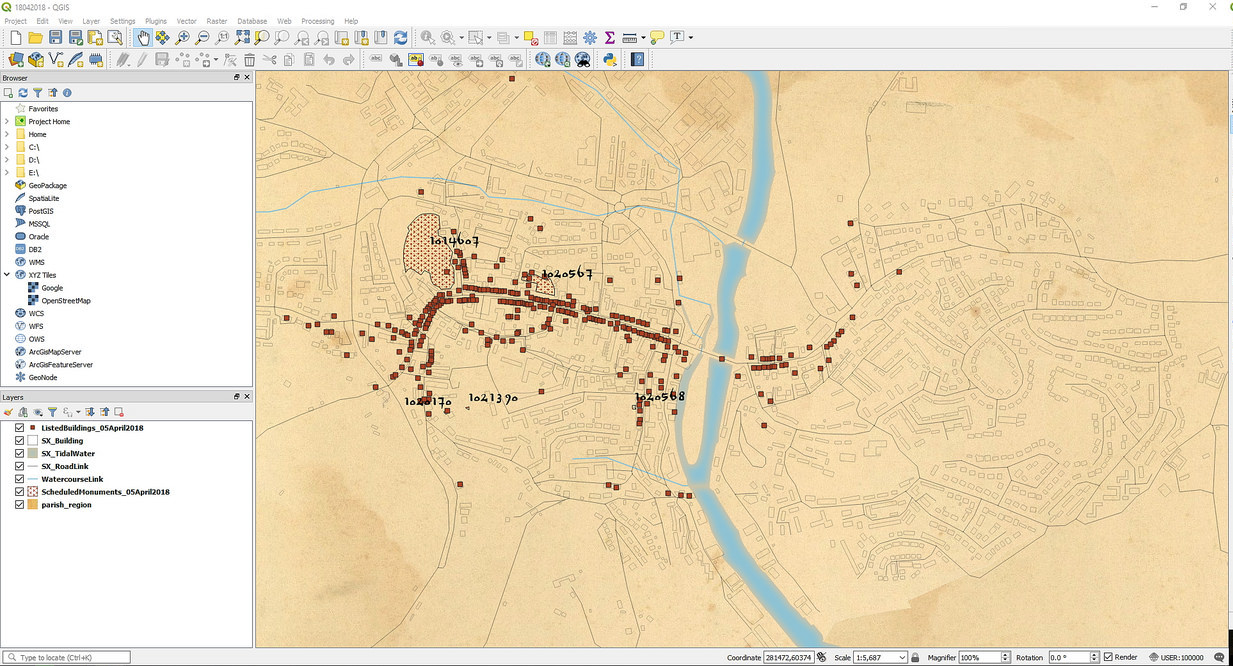
\includegraphics[width=0.8\linewidth,height=\textheight,keepaspectratio]{figure/qgis.jpg}

\subsection{References}\label{references}

\protect\phantomsection\label{refs}
\begin{CSLReferences}{1}{0}
\bibitem[\citeproctext]{ref-bailoRidingInformationCrises2024}
Bailo, F., Johns, A., \& Rizoiu, M.-A. (2024). Riding information
crises: {The} performance of far-right {Twitter} users in {Australia}
during the 2019--2020 bushfires and the {COVID}-19 pandemic.
\emph{Information, Communication \& Society}, 27(2), 278--296. DOI:
\href{https://doi.org/10.1080/1369118X.2023.2205479}{10.1080/1369118X.2023.2205479}

\bibitem[\citeproctext]{ref-bertini_galileo_1858}
Bertini, G. (1858). Galileo {Galilei} showing the {Doge} of {Venice} how
to use the telescope.
\url{https://commons.wikimedia.org/wiki/File:Bertini_fresco_of_Galileo_Galilei_and_Doge_of_Venice.jpg\#/media/File:Bertini_fresco_of_Galileo_Galilei_and_Doge_of_Venice.jpg}

\bibitem[\citeproctext]{ref-bird_natural_2009}
Bird, S., Klein, E., \& Loper, E. (2009). \emph{Natural language
processing with {Python}} (1st ed.). Cambridge, MA: O'Reilly Media.

\bibitem[\citeproctext]{ref-jockers_text_2014}
Jockers, M.L. (2014). \emph{Text analysis with {R} for students of
literature}. New York, NY: Springer.

\bibitem[\citeproctext]{ref-johnsLabellingShadowBans2024}
Johns, A., Bailo, F., Booth, E., \& Rizoiu, M.-A. (2024). Labelling,
shadow bans and community resistance: {Did} {Meta}'s strategy to
suppress rather than remove {COVID} misinformation and conspiracy theory
on {Facebook} slow the spread? \emph{Media International Australia}.
DOI:
\href{https://doi.org/10.1177/1329878X241236984}{10.1177/1329878X241236984}

\bibitem[\citeproctext]{ref-kongSlippingExtremeMixed2022}
Kong, Q., Booth, E., Bailo, F., Johns, A., \& Rizoiu, M.-A. (2022).
Slipping to the extreme: {A} mixed method to explain how extreme
opinions infiltrate online discussions. \emph{Proceedings of the
International AAAI Conference on Web and Social Media}, 16(1), 524--535.
DOI:
\href{https://doi.org/10.1609/icwsm.v16i1.19312}{10.1609/icwsm.v16i1.19312}

\bibitem[\citeproctext]{ref-manning_introduction_2008}
Manning, C.D., Raghavan, P., \& Schütze, H. (2008). \emph{Introduction
to information retrieval}. New York, NY: Cambridge University Press.

\bibitem[\citeproctext]{ref-marin_social_2011}
Marin, A., \& Wellman, B. (2011). Social network analysis: {An}
introduction. In J. Scott \& P. J. Carrington (Eds.), \emph{The {Sage}
handbook of social network analysis} (pp. 11--25). London: SAGE
Publications.

\bibitem[\citeproctext]{ref-newman_networks_2010}
Newman, M.E.J. (2010). \emph{Networks: An introduction}. Oxford: Oxford
University Press.

\bibitem[\citeproctext]{ref-salganik_bit_2018}
Salganik, M.J. (2018). \emph{Bit by bit: {Social} research in the
digital age}. Princeton, NJ: Princeton University Press.

\bibitem[\citeproctext]{ref-sarigol_online_2014}
Sarigol, E., Garcia, D., \& Schweitzer, F. (2014). Online privacy as a
collective phenomenon. \emph{arXiv Preprint arXiv:1409.6197}.
\url{http://arxiv.org/abs/1409.6197}

\bibitem[\citeproctext]{ref-scott_what_2012}
Scott, J. (2012). \emph{What is social network analysis?} London:
Bloomsbury Publishing.

\bibitem[\citeproctext]{ref-tufte_visual_2001}
Tufte, E.R. (2001). \emph{The visual display of quantitative
information} (2nd ed). Cheshire, CT: Graphics Press.

\end{CSLReferences}




\end{document}
